\documentclass[a4paper,12pt]{article}

\usepackage{graphicx}
\usepackage{amsmath}
\usepackage{float}

\begin{document}

\noindent
\begin{minipage}[t]{0.2\textwidth}

\includegraphics[width=2.5cm]{iiitb_logo.png}
\end{minipage}
\hfill
\begin{minipage}[t]{0.7\textwidth}
\raggedleft

{\Large \textbf{Pavithra Kune}}

COMETFWC069

\end{minipage}

\vspace{0.8cm}

\begin{center}
{\Large \textbf{GATE QUESTION Q36}}
\end{center}

\vspace{0.3cm}
\hrule
\vspace{0.5cm}

\begin{figure}[H]
\centering

\includegraphics[width=0.8\textwidth]{question.png}
\caption{GATE Question Q36}
\end{figure}

\tableofcontents

\newpage

\section{Components}

\begin{center}
\begin{tabular}{|c|c|c|}
\hline
Component & Specification & Quantity\
\hline
Breadboard & Standard & 1\
Arduino Uno & ATmega328P & 1\
IC 7447 & BCD to 7 Segment Decoder & 1\
7 Segment Display & Common Anode & 1\
Jumper Wires & Male-Male & As Required\
\hline
\end{tabular}
\end{center}

\subsection{Breadboard}

The breadboard is used for making temporary circuit connections.

\subsection{Arduino Uno}

Arduino Uno is used to generate the BCD inputs.

\subsection{IC 7447}

The 7447 is a BCD to Seven Segment Decoder Driver used with common anode displays.

\subsection{Seven Segment Display}

The display is used to show the output digit.

\section{Boolean Simplification}

For X=1,

[
F=\bar{Z}
]

For output 1,

[
Z=0
]

\section{Hardware Connections}

\subsection{Arduino to 7447}

\begin{center}
\begin{tabular}{|c|c|}
\hline
Arduino Pin & 7447 Pin\
\hline
D2 & A\
D3 & B\
D4 & C\
D5 & D\
\hline
\end{tabular}
\end{center}

\subsection{7447 to Seven Segment Display}

\begin{center}
\begin{tabular}{|c|c|}
\hline
7447 Output & Display Segment\
\hline
a & a\
b & b\
c & c\
d & d\
e & e\
f & f\
g & g\
\hline
\end{tabular}
\end{center}

The common anode pin of the display is connected to +5V.

\section{Software Implementation}

\begin{verbatim}
#include <Arduino.h>

void disp_7447(int D,int C,int B,int A)
{
digitalWrite(2,A);
digitalWrite(3,B);
digitalWrite(4,C);
digitalWrite(5,D);
}

void setup()
{
pinMode(2,OUTPUT);
pinMode(3,OUTPUT);
pinMode(4,OUTPUT);
pinMode(5,OUTPUT);
}

void loop()
{
int Z = 0;
int F = !Z;

if(F == 1)
disp_7447(0,0,0,1);
else
disp_7447(0,0,0,0);
}
\end{verbatim}

\section{Output}

\begin{figure}[H]
\centering
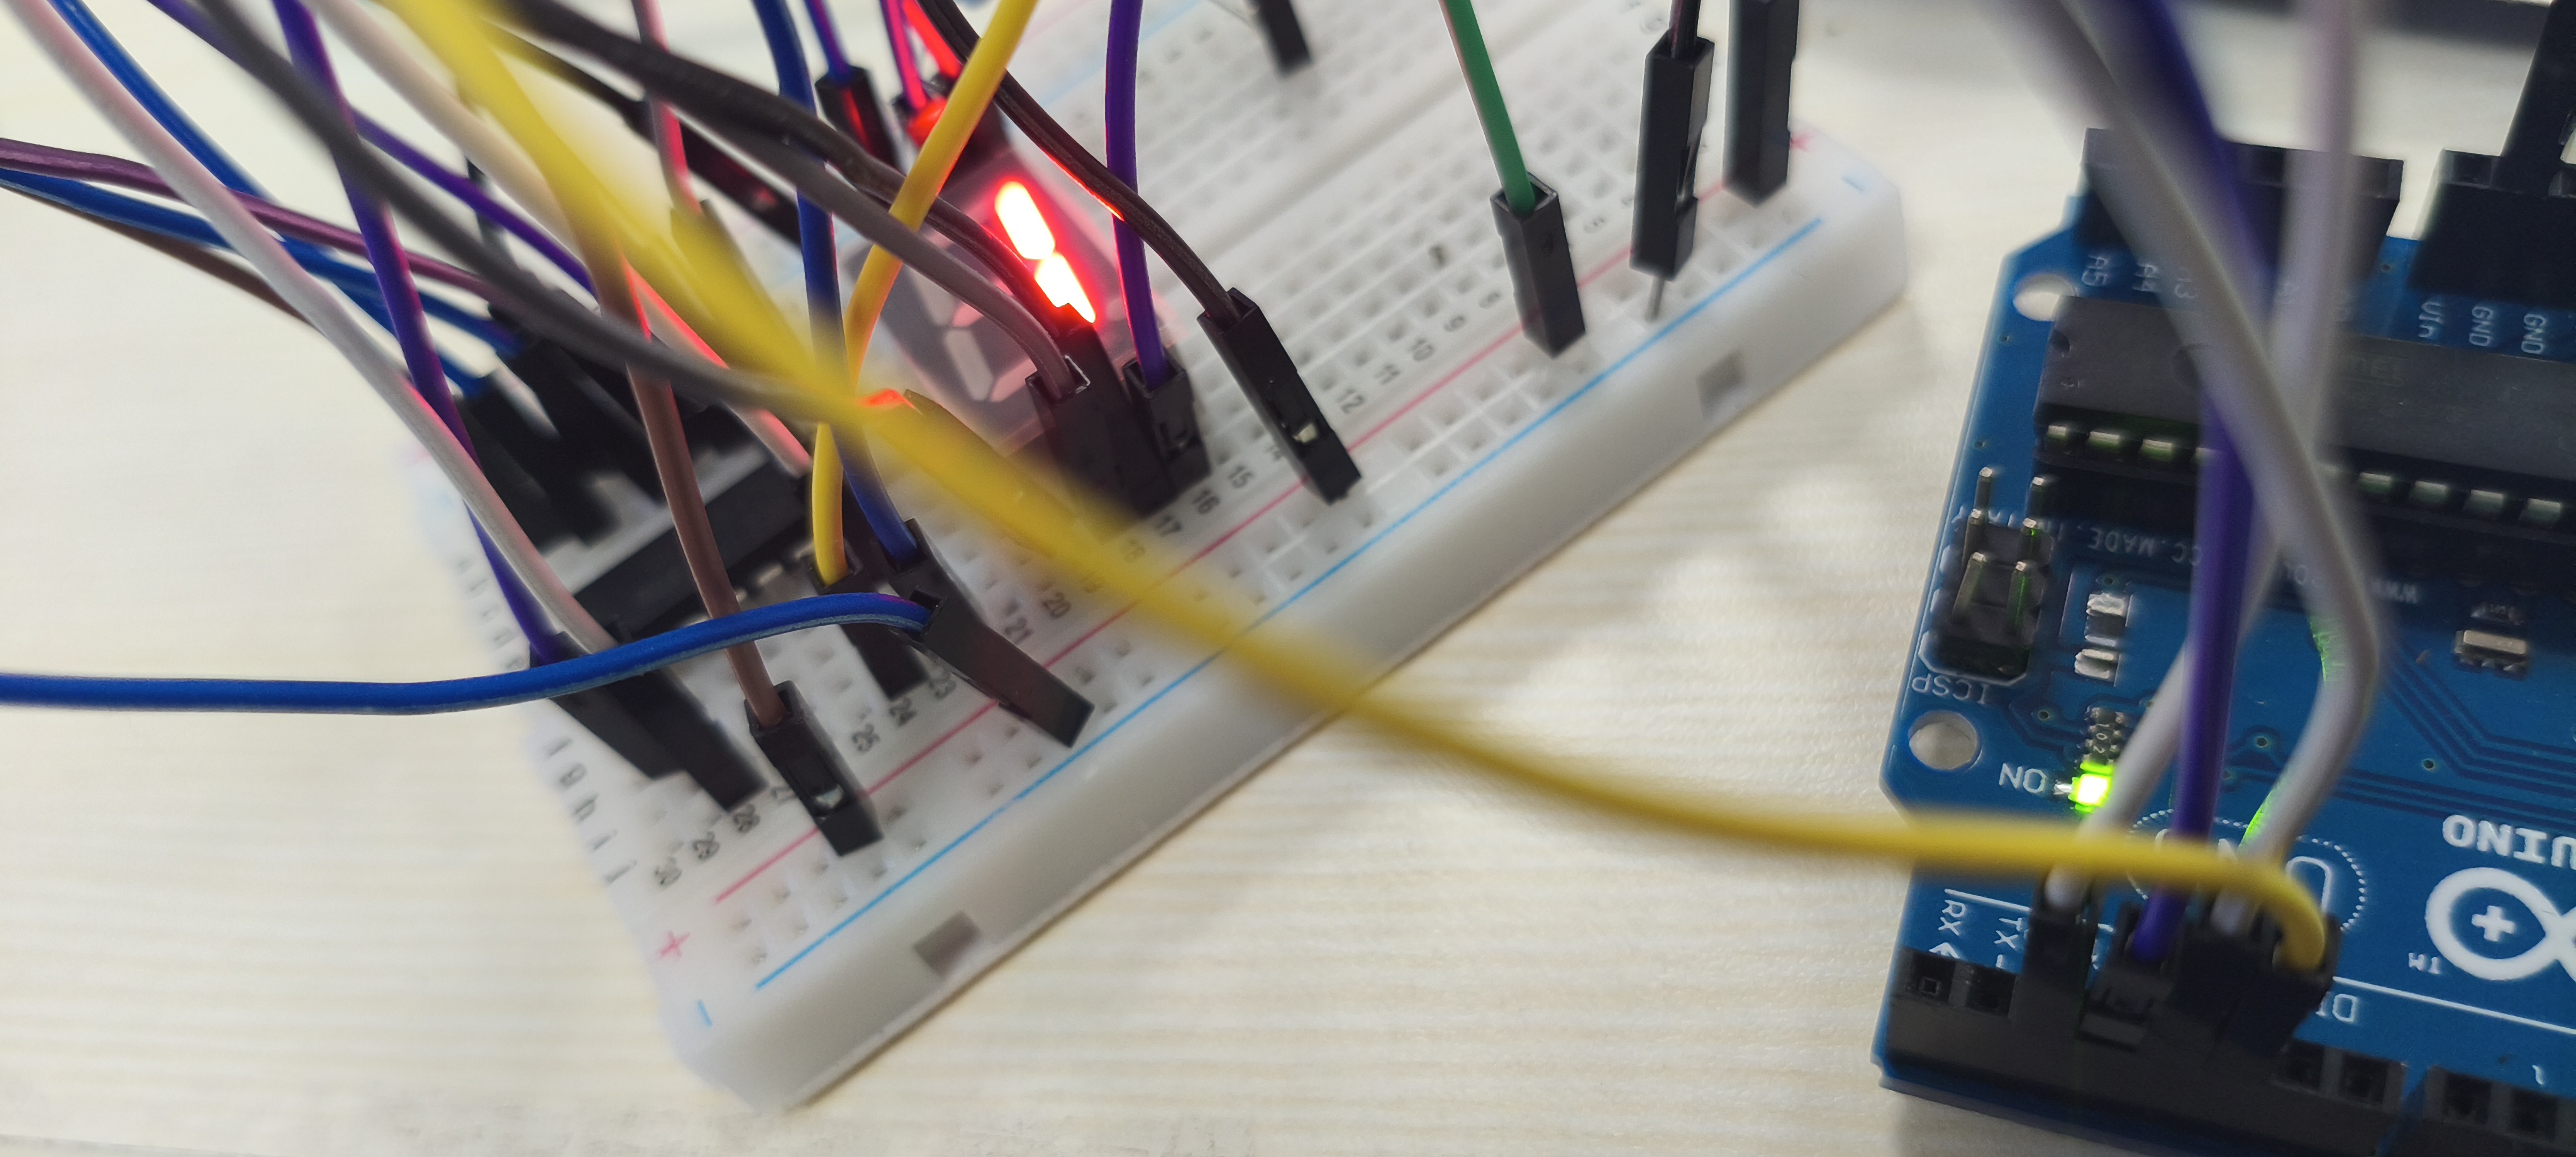
\includegraphics[width=0.5\textwidth]{output1.jpg}
\caption{Output Showing 1}
\end{figure}

\begin{figure}[H]
\centering
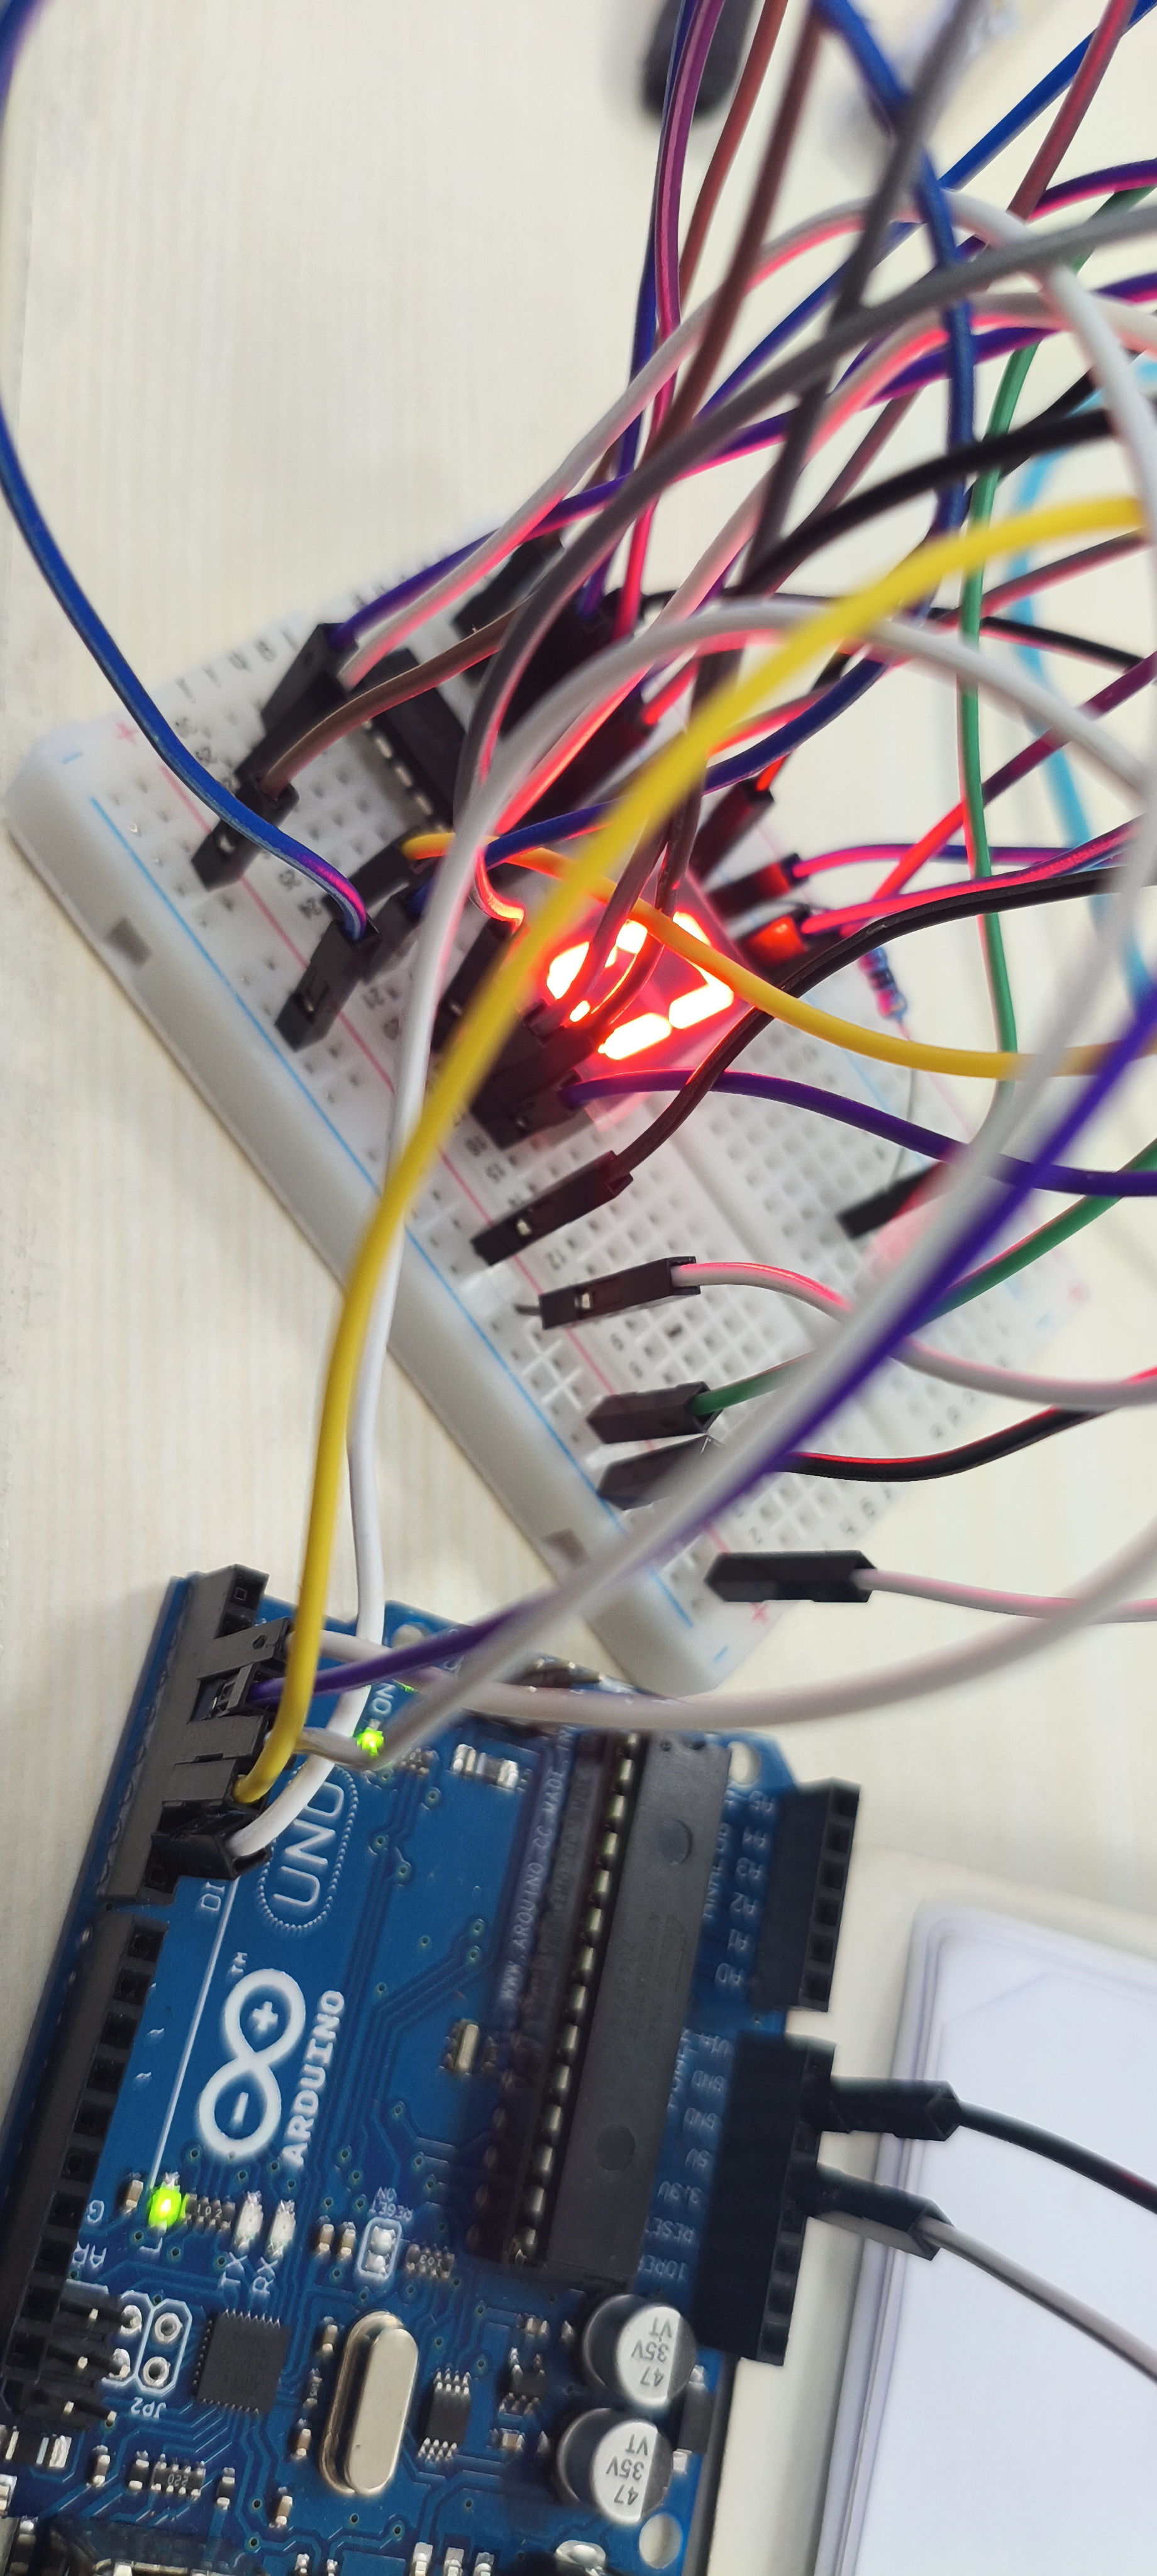
\includegraphics[width=0.5\textwidth]{output0.jpg}
\caption{Output Showing 0}
\end{figure}

\section{Result}

The given Boolean expression was implemented using Arduino Uno, IC 7447 and a common anode seven segment display.

[
F=\bar{Z}
]

Therefore,

[
Z=0
]

produces output 1 on the display.

\end{document}
